\chapter{Estado del Arte}

\section{Análisis del Estado del Arte} \label{sec:analisis_estado_arte}

Los chatbots son agentes conversacionales que pueden interactuar, a través de voz o texto, con los usuarios a través de lenguajes naturales \cite{RefWorks:RefID:36-luo2022critical}. El auge de esta tecnología en los últimos años es debido a que puede ser utilizada como mano de obra a un coste menor en una amplia gama de campos. Tal y como se indica en \cite{RefWorks:RefID:37-adamopoulou2020overview} los chatbots no están diseñados solamente para imitar y entretener a los humanos, sino que también puede diseñarse para actividades como la atención al cliente, la asistencia personal o la pedagogía entre otras. Y no hay mejor forma de asegurar el potencial de los chatbots que mostrando el aumento de inversión en \gls{IA} en el campo de las telecomunicaciones (Figura \ref{fig:inversion_chatbot}) o mostrando el aumento de publicaciones sobre chatbots (Figura \ref{fig:publicaciones_chatbot}); y viendo qué empresas están apostando por esta tecnología, como pueden ser cinco grandes empresas tecnológicas como son Google, Apple, Facebook, Microsoft y Amazon. Aunque basándonos en este párrafo de la sensación de que todas las empresas deberían disponer de chatbots, esta tecnología necesita de cierta planificación y comprensión de la tecnología, pues requiere de una gran inversión inicial, dado su gran requerimiento de información para funcionar de forma correcta.

\begin{figure}[h]
\centering
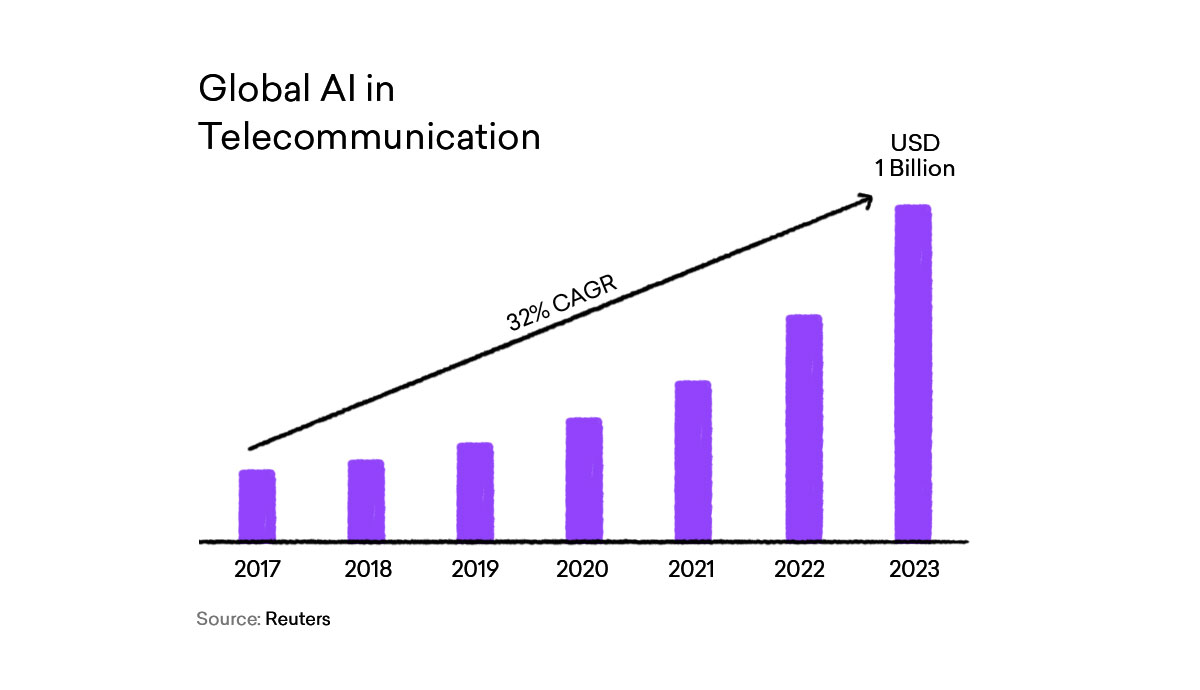
\includegraphics[width=1.0\textwidth]{imagenes/02_EstadoDelArte/inversion_chatbots.jpg}
\begin{center}
Fuente: \url{https://es.aivo.co/blog/chatbots-in-telecom}
\end{center}
\caption{Estimación de la inversión en IA en el campo de las telecomunicaciones}
\label{fig:inversion_chatbot}
\end{figure}

\begin{figure}[h]
\centering
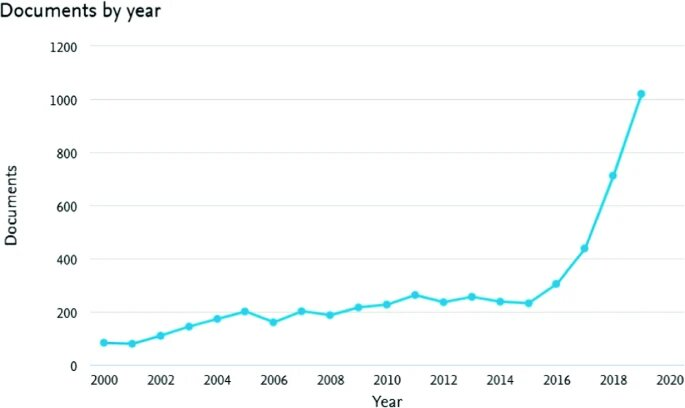
\includegraphics[width=1.0\textwidth]{imagenes/02_EstadoDelArte/publicaciones_chatbots.jpg}
\begin{center}
Fuente: \url{https://link.springer.com/chapter/10.1007/978-3-030-49186-4_31}
\end{center}
\caption{Historial de las publicaciones sobre temas relacionados con chatbots}
\label{fig:publicaciones_chatbot}
\end{figure}

Aunque es una tecnología en auge y con mucho potencia en este momento, hay aspectos de ella que todavía no están lo suficientemente desarrollados como para decir que se trata de una tecnología del todo madura. Estas carencias están sobre todo enfocadas en tres puntos.
En primer lugar, nos encontramos con el problema que aparece nada más empezar, y es la carencia de un esquema de clasificación de chatbots, dado que no se ha definido una clasificación global. La clasificación más extendida es la clasificación según el mecanismo de recuperación y de generación de respuestas, donde destacan los chatbots que hacen uso de bases de conocimientos estáticas, es decir, chatbots basados en reglas; y los chatbots que hacen uso de mecanismos de aprendizaje e inferencia adaptativos, es decir, los chatbots basados en \newline\gls{IA}, los cuales son el objetivo de la mayoría de los desarrollos actuales. En segundo punto, las revisiones están desactualizadas en el ámbito de la generación de respuestas dado el rápido avance de las técnicas computacionales. En tercer punto, también las revisiones no están muy centradas en la aplicación empresarial de los chatbots ni en su usabilidad, sino que más bien están centradas en el aspecto técnico, lo cual complica su desarrollo por parte de trabajadores ajenos al mundo de la informática y/o de la \gls{IA}.

La estructura de los chatbots ha ido evolucionando y extendiéndose. Originalmente, la estructura de los chatbots era la descrita por Abdul-Kader y Woods \cite{RefWorks:RefID:36-luo2022critical}, donde se podía reconocer tres componentes: interfaz, un clasificador y un graphmaster. Esta estructura está muy desactualizada a día de hoy, ya que en la estructura original la interfaz solo tenía previstas entradas en forma de texto, pero hoy en día las entradas son de tipo multimedia, por lo que es necesario actualizar la interfaz a una interfaz multimedia, y añadir un nuevo componente a la estructura, encargado de manejar esas entradas multimedia y convertirlas en entradas de texto que se puedan manejar para generar respuestas; además dado el auge de los chatbots basados en generación, a día de hoy el componente del graphmaster no tiene sentido, dado que las respuestas se generan utilizando modelos pre entrenados realizando inferencias basándose en las entradas, por lo que tener un manejador para el almacenamiento de conocimiento deja de tener sentido. Por lo tanto, en la estructura el graphmaster debe ser actualizado por un modelo generador de respuestas. Aplicando todas estas actualizaciones sobre la estructura original de Abdul-Kader y Woods, obtenemos la estructura actual de los chatbots, que se muestra en la Figura \ref{fig:estructura_state_of_art}. Finalmente, tenemos cuatro componentes: la interfaz, un procesador multimedia, un análisis de entrada multimodal y un generador de respuestas.

\begin{figure}[h]
\centering
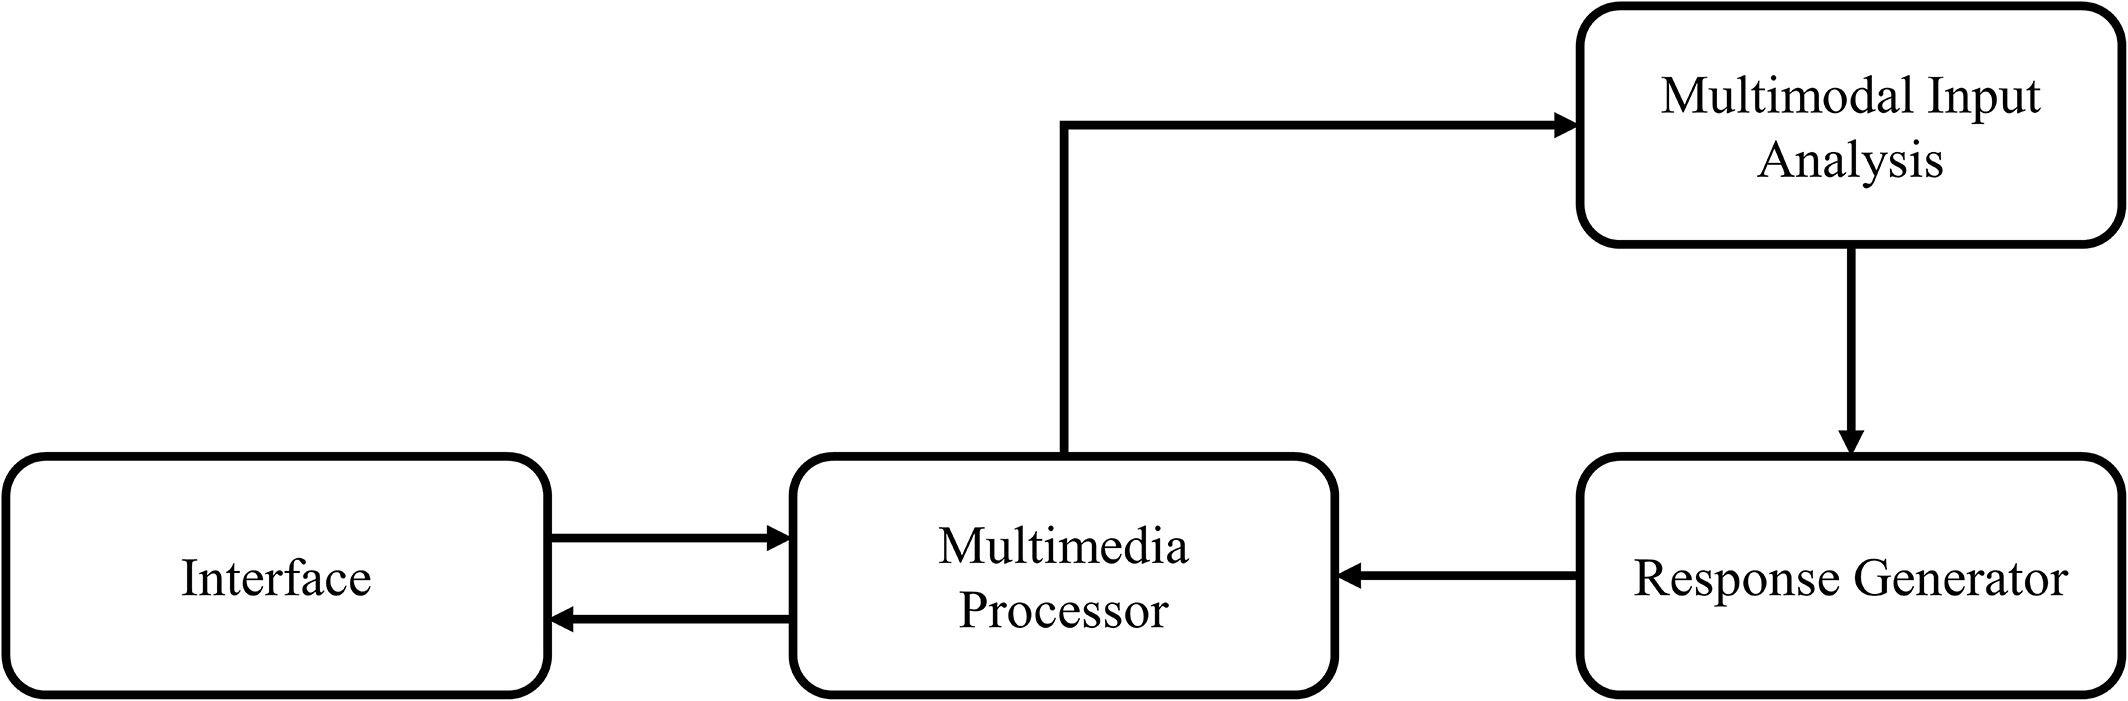
\includegraphics[width=0.8\textwidth]{imagenes/02_EstadoDelArte/estructura_state_of_art.jpg}
\begin{center}
Fuente: A critical review of state-of-the-art chatbot designs and applications \cite{RefWorks:RefID:36-luo2022critical}
\end{center}
\caption{Estructura de los chatbots actuales}
\label{fig:estructura_state_of_art}
\end{figure}

Un componente que se muestra en la Figura \ref{fig:estructura_state_of_art} y que no se ha mencionado explícitamente cuál es su labor es el análisis de entrada multimodal. Este análisis efectúa un pretratamiento de los datos de entrada, hoy en día se intenta mejorar este componente con \gls{NLU} (NLU).

En el caso de los chatbots basados en la recuperación, el generador de respuestas desempeña el mismo papel que el graphmaster, ya que almacena y recupera las respuestas; mientras que en el caso de los chatbots basados en la generación, genera una salida a partir de la entrada que ha sido transferida desde la unidad de pretratamiento \cite{RefWorks:RefID:36-luo2022critical}.

Centrándonos en el componente del generador de respuestas, a día de hoy se utilizan distintas técnicas para implementar este componente. Las técnicas más destacadas son las siguientes:

\begin{itemize}
\item \textbf{Template:} Esta técnica se compone de patrones y plantillas formando pares con ellos. Para generar las respuestas se busca el patrón que más concuerde con la entrada recibida, y una vez se haya elegido un patrón se devuelve la plantilla asociada al mismo. El lenguaje que más destaca en esta técnica es AIML \footnote{\url{http://www.aiml.foundation}}. La desventaja de tener que crear los archivos AIML se puede suplir mediante la extracción automática de conocimientos, reduciendo el trabajo manual. Los chatbots basados en plantillas son sencillos de producir, por lo tanto, son una opción popular para chatbots sencillos a pequeña escala.
\item \textbf{Corpus:} Son una buena técnica como alternativa a los templates cuando se están construyendo chatbots a gran escala, debido a que con los templates al aumentar de escalas aumenta el número de patrones y trae consigo búsquedas más lentas lo que ralentiza la generación de respuestas. Existen dos tipos de chatbots basados en Corpus, un tipo de chatbots basados en corpus que no selecciona cuidadosamente el conocimiento y otro que si lo hace. El tipo que selecciona cuidadosamente el conocimiento se puede implementar mediante bases de datos o mediante modelos de ontología, los modelos de ontología tienen una gestión más flexible del conocimiento que las bases de datos, la generación en este tipo de chatbots se realiza también con búsqueda pero esta vez en las estructuras mencionadas anteriormente. El tipo que no selecciona cuidadosamente el conocimiento transforma las palabras en vectores que representan los significados semánticos de las palabras en un espacio multidimensional, la generación en este tipo de chatbots se realiza mediante el cálculo de la distancia entre los pares de entrada del usuario y de consulta-respuesta, se empareja la consulta con la menor distancia y se selecciona su correspondiente respuesta como salida. Debido a la gran capacidad de gestión del conocimiento, varias aplicaciones que requieren un conocimiento formal del dominio utilizan chatbots basados en corpus \cite{RefWorks:RefID:36-luo2022critical}.
\item \textbf{Intent:} Los chatbots basados en intenciones se emplean ampliamente para los sistemas orientados a tareas que presentan diálogos de varios turnos \cite{RefWorks:RefID:36-luo2022critical}. Una intención representa un mapeo entre lo que dice el usuario y la acción que debería ejecutar el chatbot. El emparejamiento de las entradas con las distintas intenciones se hace de una forma distinta a la vista anteriormente, dado que ahora debemos emparejar los elementos semántico en vez de la frase completa. Puesto que la entrada es una frase, en el caso de esta técnica es necesario añadir adicionalmente un componente de análisis de entrada multimodal (SLU), dentro de él se efectúa un análisis semántico de las entradas, para este análisis se suelen usar \gls{NLU}. Una vez tenemos los elementos semánticos de la entrada se procede a emparejar la entrada con una intención o dicho de otra manera, se procede a efectuar una clasificación para saber a qué intención pertenece la entrada, esta clasificación se suele hacer mediante técnicas de aprendizaje automático. Otra característica de este tipo de chatbots es la existencia de estados, debido a que son chatbots orientados a tareas; los cuales determinan el momento de la conversación en el que nos encontramos, que intenciones han sido ejecutadas, y cuáles pueden ser elegidas para ejecutar posteriormente. El manejo de los estados se compone de dos tareas, por un lado, la obtención del estado actual del diálogo, para lo cual se utilizan técnicas de \gls{DST}; y, por otro lado, el procesamiento del estado del diálogo para determinar a que estado se va a pasar el diálogo, para esta tarea se utilizan técnicas de \gls{DPO}. Las dos técnicas mencionadas son necesarias para establecer la secuencia de los diálogos. Las bases de conocimiento de los generadores de respuestas en los chatbots basados en intenciones están compuestas principalmente de frases de entrenamiento, intenciones y respuestas. Para generar las respuestas se analiza semánticamente las entradas en el módulo SLU, posteriormente se emplea el módulo \gls{DST}para estimar el estado de los diálogos actuales y finalmente se emplea el módulo \gls{DPO} para determinar las acciones y respuestas.

Para un mejor entendimiento de esta compleja estructura se dispone de la Figura \ref{fig:estructura_intent}.

\begin{figure}[h]
\centering
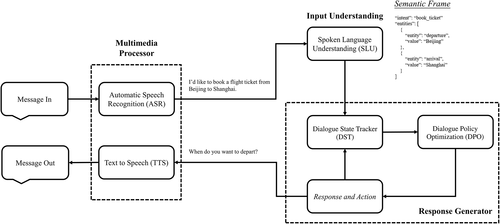
\includegraphics[width=0.8\textwidth]{imagenes/02_EstadoDelArte/estructura_intent.png}
\begin{center}
Fuente: A critical review of state-of-the-art chatbot designs and applications \cite{RefWorks:RefID:36-luo2022critical}
\end{center}
\caption{Estructura de los chatbots basados en intenciones}
\label{fig:estructura_intent}
\end{figure}

Muchas de las grandes plataformas actualmente están orientadas a la creación de chatbots de este tipo, como puede ser la plataforma de Google con Dialogflow \footnote{\url{https://dialogflow.cloud.google.com}} (originalmente llamado Api.ai) o la plataforma de código abierto de Rasa. \footnote{\url{https://rasa.com/}}.
\item \textbf{Red neuronal recurrente (RNN):} Los chatbots creados con esta técnica dejarán de estar basados en la recuperación, como pasaba en las tres anteriores técnicas, si no que estarán basados en la generación, pero esto que quiere decir, en definitiva quiere decir que la generación de las respuestas no se realizará mediante búsquedas en alguna estructura y sustitución mediante pares consulta-respuesta. La generación de las respuestas se efectúa mediante inferencias con modelos de redes neuronales recurrentes. Estos chatbots, a diferencia de los chatbots basados en intenciones, no están orientados a las tareas y esto deriva del problema que conllevan las redes neuronales, y no es otro que las redes convierten al chatbot en una caja negra, esto quiere decir que la respuesta del chatbot ante cierta entrada es incierta incluso para su creador, este inconveniente se convierte en una ventaja si orientamos a los chatbots al chat, dado que esta incertidumbre en la respuesta da una gran sensación de naturalidad y creatividad durante la conversación, por lo que son apropiados para actividades relacionadas con el entretenimiento y la salud mental entre otras. Estos chatbots se han visto muy potenciados en los últimos años debido al rápido desarrollo del aprendizaje profundo. Uno de los mayores hitos en el aprendizaje profundo ha sido la creación de GPT-3 \footnote{\url{https://openai.com/blog/openai-api}} creado por la empresa OpenAI, el cual es un nuevo modelo de \gls{IA} que permite generar lenguaje escrito. Como se ha mencionado anteriormente, ya no se realiza recuperación para la generación de respuestas, por lo tanto, las bases de conocimiento de los chatbots basados en RNN estarán compuestas de los conjuntos de datos de entrenamiento. El resultado de los chatbots basados en la generación depende de la especificación del modelo, los conjuntos de datos de entrenamiento, el proceso de entrenamiento y la entrada del usuario \cite{RefWorks:RefID:36-luo2022critical}.
\item \textbf{Aprendizaje por refuerzo (RL):} Este tipo de chatbots suelen estar basados en la recuperación y utilizan plenamente el contexto de entrada para la búsqueda de respuestas óptimas \cite{RefWorks:RefID:36-luo2022critical}. Dado que se basan en la recuperación, en sus bases de conocimientos hay pares de consulta-respuesta predefinidos. El método RL se basa principalmente en el \gls{Markov}. Al igual que pasaba en los chatbots basados en templates, en los chatbots basados en RL se usan representaciones vectoriales, en concreto el estado del chatbot es una representación vectorial de un turno de conversación. Este vector puede contener la respuesta derivada de la entrada o adicionalmente puede contener el acto de diálogo, el sentimiento del usuario y el enunciado genérico del usuario. El contexto de la comunicación forma una secuencia de estados. Aunque es una técnica basada en la recuperación, esta recuperación es distinta a la descrita en las anteriores técnicas, en el caso de esta técnica se emplea una política para encontrar la respuesta adecuada, esta política debe ser bien entrenada para lo que son necesarios diálogos predefinidos. Este tipo de chatbots se pueden utilizar para secciones de "Preguntas frecuentes".
\item \textbf{Enfoques híbridos:} \label{enfoque_hibrido} El intento de combinar varias técnicas para suplir las desventajas de ambas con las ventajas de cada técnica es algo que se ha intentado en una multitud de ámbitos, y este no iba a ser menos. En \cite{RefWorks:RefID:36-luo2022critical} se hace referencia a una serie de propuestas de diferentes investigadores. Una de ellas puede ser la realizada por Li Wu y Wu Wu, los cuales propusieron un marco de correspondencia secuencial basado en una RNN. El marco considera las relaciones entre los enunciados anteriores y las respuestas candidatas y selecciona las respuestas óptimas para el contexto.
\end{itemize}

Si nos fijamos en la técnica utilizada para crear el chatbot podemos obtener una buena clasificación de los mismos.

Una vez estudiada la estructura actual de los chatbots. A continuación voy a exponer algunas de las posibles aplicaciones que pueden tener los distintos chatbots.

\begin{itemize}
\item \textbf{Atención al cliente para el comercio electrónico:} Puede que sea la aplicación más usada. Dado el gran crecimiento del sector, se ha producido un elevado aumento de la carga de trabajo. Como se ha indicado anteriormente, por ejemplo, en el caso de los chatbots basados en intenciones, los chatbots son capaces de reducir la carga de trabajo y consecuentemente también reduce los costes humanos. La calidad del servicio proporcionado por estos chatbots está en continua mejora debido a la dificultad de manejar peticiones muy complejas por parte del usuario y otros problemas como el amplio dominio necesario para contestar de forma correcta durante toda la conversación y no solamente para contestar, sino también para realizar un servicio agradable para el usuario.
\item \textbf{Asistencia personal:} Esta aplicación está muy extendida y es utilizada asiduamente por multitud de personas. Los chatbots de asistencia personal pueden emplearse para aumentar la eficiencia del trabajo o para gestionar la vida cotidiana del usuario. Un posible ejemplo podría ser Siri \footnote{\url{https://www.apple.com/es/siri}}, que es un chatbot incorporado en todos los dispositivos iPhone.
\item \textbf{Asistencia sanitaria:} Esta clase de chatbots actúan como asistentes médicos para el diagnóstico de enfermedades. La comprensión de los síntomas del paciente es primordial en el proceso de detección de la enfermedad, y una de las principales funciones de estos chatbots es recoger suficiente información de los pacientes \cite{RefWorks:RefID:36-luo2022critical}. Aunque en los aspectos médicos la última palabra la tiene un profesional humano, los chatbots puede realizar diagnósticos previos rápidamente dada su inmenso conocimiento al que se puede acceder en un instante, cosa que no sucede con los humanos, lo que ralentiza el diagnóstico. Esta enorme base de conocimiento es muy importante en la medicina debido al vasto dominio de este campo y el cual está en continuo crecimiento y mejora.
\item \textbf{Pedagogía:} Estos chatbots están diseñados para ayudar al aprendizaje. Dado que la función principal de los chatbots es comunicarse con los usuarios, el aprendizaje de idiomas ha sido una de las principales vías perseguidas \cite{RefWorks:RefID:36-luo2022critical}, ya que el aprendizaje de idiomas está a la orden del día de todo el mundo. Estos chatbots son útiles para enseñar a usuarios mediante conocimientos de expertos, sin que sea necesario una ingente cantidad de expertos para enseñar, puesto que esta cantidad de expertos en ciertos campos y lugares no está disponible.
\end{itemize}

En todas estas aplicaciones existe el problema de la seguridad de los datos necesarios por el chatbot, este aspecto está muy presente en los últimos años debido a los múltiples casos publicados sobre falta de seguridad con los datos de los usuarios. De cara al futuro se pretende que aumente la seguridad de estos datos. Una solución de reciente desarrollo para la problemática de la privacidad de los datos, es el aprendizaje federado. Tal y como indica Karen Hao \cite{RefWorks:RefID:42-hao1970aprendizaje}: "Aprendizaje federado: la nueva arma de IA para asegurar la privacidad". Este tipo de aprendizaje influye en una de las partes críticas de la privacidad de los datos, y es el traspaso de los datos entre dos ubicaciones. El aprendizaje federado evita ese traspaso de los datos, entrenando pequeños modelos en cada ubicación donde se encuentren los datos, y posteriormente traspasando estos pequeños modelos y finalmente combinando todos estos modelos en un modelo maestro único. Un ejemplo claro de aplicación de estos algoritmos lo da Karen Hao \cite{RefWorks:RefID:42-hao1970aprendizaje}, y es su uso en el ámbito de la sanidad, dado que para elaborar modelo de IA en la salud es necesario traspasar la información almacenada en cada hospital para poder elaborar ese modelo; pero con el aprendizaje federado se podría evitar ese traspaso crítico de información.

Llegados a este punto en el que ya hemos analizado el estado actual de los chatbots, únicamente nos queda analizar cuál es la dirección de las futuras investigaciones en este sector. Estas investigaciones estarán centradas en paliar las deficiencias y en mejorar aún más las capacidades actuales.

Uno de los principales problemas de los chatbots es la ingente cantidad de datos que necesitan para empezar a funcionar. Actualmente, este conocimiento es almacenado en estructuras de distinto tipo, sin tener un esquema unificado. Esta variedad de bases de conocimiento distintas dificulta la creación de nuevos chatbots al no poder reutilizar datos utilizados en chatbots anteriores. Una posible futura mejora sería la estandarización de la gestión del conocimiento para poder realizar esta transferencia de datos entre chatbots de forma eficiente. Una solución a este problema, la cual es ampliamente empleada, es el empleo de modelos pre entrenados. Estos modelos son simplemente modelos que han sido entrenados con un cierto tipo de información, los cuales son modelos simples que podemos usar como apoyo para la creación de modelos más complejos. Esta manera de elaborar los modelos sigue la filosofía del Transfer learning, la cual consiste en transferir conocimientos adquiridos con la resolución de ciertos problemas en la resolución de otros problemas distintos a los usados en un principio.

Un aspecto analizado anteriormente es la generación de las respuestas, este aspecto aunque ha sufrido un gran desarrollo en los últimos años, todavía no ha llegado a alcanzar su máximo nivel, esto se puede comprobar simplemente con ver, tal y como indica \cite{RefWorks:RefID:36-luo2022critical}, que todavía nadie ha ganado el premio de oro del Premio Loebner, el concurso de pruebas Turing más famoso en el ámbito de los chatbots. Las futuras investigaciones están orientadas a la mejora de las técnicas de aprendizaje profundo. Estas técnicas son entre otras las \gls{GAN} (GAN), este tipo de redes está muy extendido en el mundo de la visión por computador, pero todavía no se ha llegado a conseguir una integración de esta técnica en el mundo de los chatbots.

Un aspecto de los chatbots que todavía tiene mucho potencial por explotar es sin duda la interfaz. Hasta ahora solamente hemos indicado que se están utilizando interfaces multimodales. Pero no se está sacando todo el partido a este tipo de interfaces, dado que actualmente únicamente se realiza una conversión de todo tipo de entradas a una entrada en formato de texto. Pero las entradas multimodales contienen información adicional a la que se extrae hoy en día, como puede ser el lenguaje no verbal durante una conversación por voz. Este lenguaje no verbal proporciona mucha información que puede ayudar a la generación de respuestas y a tener un mejor contexto de la conversación. Para que toda esta información no se desperdicie se debe avanzar en la investigación para la extracción de esta información. Otro aspecto de la interfaz donde es necesaria la investigación es la devolución de la respuesta a través de la interfaz, ya que hasta ahora estábamos hablando de como se debía mejorar la entrada de información en la interfaz. La devolución de esta información se puede efectuar de muchas maneras, escrita, por voz, etc. Lo verdaderamente importante en la devolución de la respuesta es que el usuario perciba esa respuesta con facilidad, con una buena estética que atraiga la atención del mismo. Una de las líneas de futuras investigaciones son los avatares 3D, es decir, la respuesta es devuelta por voz, pero lleva añadida la gesticulación de un avatar 3D.

Una dirección en la que se pueden realizar futuras investigaciones son las aplicaciones del chatbot. Dado el auge del \gls{IoT} (IoT) hoy en día hay todo un campo donde integrar los chatbots para mejorar el servicio a los usuarios, como pueden ser los coches inteligentes, los hogares inteligentes, y muchos más.

Por último, tal y como se ha indicado anteriormente, uno de los grandes problemas actualmente de los chatbots es la falta de seguridad con los datos, este es un aspecto crucial en todas las futuras investigaciones.

\section{Herramientas para el desarrollo del chatbot}

Hay dos caminos para crear un chatbot, por un lado, usando cualquier lenguaje de programación como Java, Python, C++, etc; y, por otro lado, usando plataformas para el desarrollo de chatbots. En este apartado voy a analizar distintas herramientas para el desarrollo de mi chatbot.

Un aspecto a tener en cuenta a la hora de elegir una plataforma para desarrollar un chatbot es que existen dos elementos en esta creación.

\begin{itemize}
\item \textbf{Bot Frameworks}: son las plataformas encargadas de la creación y el alojamiento de los chatbots.
\item \textbf{Bot Platforms}: son los entornos y aplicaciones donde van a ser desplegados los chatbots para su uso por parte de los usuarios.
\end{itemize}

A la hora de elegir la plataforma donde desarrollar el chatbot habrá que tener en cuenta que tanto el Bot Framework como el Bot Platform elegidos se adecuan a los requisitos del chatbot a crear.

Una posible clasificación de las plataformas puede ser basándonos en el modo de creación de los chatbots. Dentro de esta clasificación encontramos las siguientes plataformas:

\begin{itemize}
\item \textbf{Plataformas visuales}
\item \textbf{Plataformas conversacionales}
\item \textbf{Plataformas programables}
\end{itemize}

\subsubsection*{Plataformas visuales}

En estas plataformas no es necesario tener conocimientos técnicos para producir un chatbot. Por esta razón son las plataformas ideales para personas que no tienen conocimientos en programación o \gls{IA}. Algunos ejemplos de este tipo de plataformas pueden ser: Chatfuel y Octane AI. Esta simpleza en la creación del chatbot afecta en la posible complejidad que pueda tener el chatbot, por lo tanto, no son la mejor opción para chatbots con cierta complejidad, pero si para chatbots muy simples.

\subsubsection*{Plataformas conversacionales}

En estas plataformas es posible la creación de chatbots algo más complejos que en las plataformas visuales. Estos chatbots son capaces de mantener una conversación con un usuario, pero que a diferencia de los anteriores chatbots, esta conversación no tiene un objetivo específico. Un posible ejemplo de este tipo de plataformas puede ser AIML, aunque AIML no es en sí una plataforma sino más bien un lenguaje de programación, sí se convierte en una plataforma si se combina el lenguaje con alguna plataforma donde se permita al menos el alojamiento del chatbot. Este tipo de plataformas ya no está orientado a usuarios sin conocimientos técnicos, sino más bien a usuarios que tengan cierto nivel técnico y que busquen crear chatbots con cierta complejidad, pero que no tengan mucha escala.

\subsubsection*{Plataformas programables}

En estas plataformas se pueden generar desde los chatbots más simples hasta los más complejos. Para poder aumentar la complejidad se hace uso de técnicas de \gls{IA} junto a las técnicas que ya se utilizaban en las anteriores plataformas, y aumenta la posibilidad de interactuar con servicios externos a la plataforma como pueden ser bases de datos y muchos más servicios. Algunos ejemplos de este tipo de plataformas pueden ser: Google Dialogflow, Microsoft Bot Framework e IBM Watson. \newline\newline

En cuanto a la implementación de chatbots mediante lenguajes de programación, es una herramienta únicamente disponible para personas con los suficientes conocimientos técnicos, no es una opción para aquellas personas que no tengan conocimientos técnicos en el ámbito de la informática.

En la actualidad se dispone de un número elevado de herramientas capaces de producir chatbots de diferentes complejidades. De entre este número elevado de herramientas he seleccionado unas cuantas para analizarlas en detalle como posibles herramientas con las que generar mi chatbot. En esta lista de herramientas no se encuentra ninguna plataforma visual dado que no posibilitan la complejidad necesaria para generar mi chatbot.

Las herramientas analizadas son las siguientes:

\begin{itemize}
    \item AIML
    \item IBM Watson
    \item Google Dialogflow
    \item Rasa Stack
    \item GPT-3
    \item BlenderBot
\end{itemize}

Para consultar la información extraída de cada una de las herramientas, la cual ha ayudado en la elección de una de ellas para el desarrollo del chatbot, debes consultar el Apéndice \ref{carac_herramientas_anali}.


\section{Comparativa de las herramientas}

Después de revisar las distintas herramientas, es hora de compararlas para facilitar la elección de una ellas para el desarrollo del proyecto. En primer lugar, se hará una comparación de pros y contras de todas las herramientas (Tabla \ref{tab:pros_contras_plataformas}), y seguidamente se mostrará una tabla (Tabla \ref{tab:carac_plataformas}) con una serie de características, indicando cuáles están presentes en las distintas herramientas.


\begin{table}[h]
\centering
\resizebox{\textwidth}{!}{%
\begin{tabular}{c|l|l|}
\cline{2-3}
\multicolumn{1}{l|}{} &
  \multicolumn{1}{c|}{\cellcolor[HTML]{FFFC9E}\textbf{PROS}} &
  \multicolumn{1}{c|}{\cellcolor[HTML]{FFFC9E}\textbf{CONTRAS}} \\ \hline
\multicolumn{1}{|c|}{\cellcolor[HTML]{FFCCC9}\textbf{AIML}} &
  \begin{tabular}[c]{@{}l@{}}- Multilenguaje\\ - El chatbot no es una caja negra\\ - Lenguaje de programación simple\\ - Posibilidad de conexión con API's propias\\ - Muchas funcionalidades de forma gratuita\end{tabular} &
  \begin{tabular}[c]{@{}l@{}}- Alto gasto de tiempo en la creación del agente conversacional\\ - Necesidad de una cuenta de pago usando servicios web\\ - No es una plataforma en la nube\\ - Conversaciones poco naturales y poco flexibles\end{tabular} \\ \hline
\multicolumn{1}{|c|}{\cellcolor[HTML]{FFCCC9}\textbf{IBM Watson}} &
  \begin{tabular}[c]{@{}l@{}}- Posibilidad de crear chatbots muy complejos\\ - Gran cantidad de conexiones con API's de mucha calidad\\ - Editor de arrastrar y soltar\\ - Facilidad de desplegar el chatbot en muchos canales importantes\\ - Es una plataforma en la nube\end{tabular} &
  \begin{tabular}[c]{@{}l@{}}- Necesidad de una cuenta de pago para crear chatbots complejos\\ - Enfocado para el mundo empresarial\\ - El chatbot es una caja negra\end{tabular} \\ \hline
\multicolumn{1}{|c|}{\cellcolor[HTML]{FFCCC9}\textbf{Dialogflow}} &
  \begin{tabular}[c]{@{}l@{}}- Posibilidad de crear chatbots muy complejos sin necesidad de pago\\ - Posibilidad de conexión con un servidor web de forma gratuita\\ - Facilidad de desplegar el chatbot en muchos canales importantes\\ - Creación de chatbots usando solamente frases y entidades\\ - Es una plataforma en la nube\end{tabular} &
  \begin{tabular}[c]{@{}l@{}}- Para hacer agentes muy complejos es necesario gastar tiempo \\ en la creación del servidor\\ - Se necesita tener cierto conocimiento de la plataforma para \\ sacar todo su potencial\\ - Calidad regular en la documentación\\ - Parte del chatbot es una caja negra\end{tabular} \\ \hline
\multicolumn{1}{|c|}{\cellcolor[HTML]{FFCCC9}\textbf{Rasa Stack}} &
  \begin{tabular}[c]{@{}l@{}}- Documentación de calidad\\ - El chatbot no es una caja negra\\ - Facilidad de desplegar el chatbot en muchos canales importantes\\ - Posibilidad de crear chatbots muy complejos\end{tabular} &
  \begin{tabular}[c]{@{}l@{}}- Necesidad de alto nivel técnico\\ - Plataforma en desarrollo\\ - Necesidad de mucho tiempo para la creación del chatbot\\ - No es una plataforma en la nube\end{tabular} \\ \hline
\multicolumn{1}{|c|}{\cellcolor[HTML]{FFCCC9}\textbf{GPT-3}} &
  \begin{tabular}[c]{@{}l@{}}- Posibilidad de crear chatbots muy complejos\\ - Chatbots con una conversación muy natural\\ - Buena documentación\end{tabular} &
  \begin{tabular}[c]{@{}l@{}}- Necesidad de conocimientos técnicos\\ - Necesidad de pago para hacer uso de los servicios\\ - Necesidad de una solución para mantener el contexto\\ - Requiere de un conjunto de datos para poder adaptar el \\ chatbot a su dominio\\ - Requiere de una plataforma aparte para el despliegue\end{tabular} \\ \hline
\multicolumn{1}{|c|}{\cellcolor[HTML]{FFCCC9}\textbf{BlenderBot}} &
  \begin{tabular}[c]{@{}l@{}}- Posibilidad de crear chatbots muy complejos\\ - Chatbots con una conversación muy natural\\ - Uso gratuito\\ - Buena documentación\end{tabular} &
  \begin{tabular}[c]{@{}l@{}}- Necesidad de conocimientos técnicos\\ - Necesidad de una solución para mantener el contexto\\ - Requiere de un conjunto de datos para poder adaptar el \\ chatbot a su dominio\\ - Requiere de una plataforma aparte para el despliegue\end{tabular} \\ \hline
\end{tabular}%
}
\caption{Comparativa de pros y contras de las herramientas de desarrollo}
\label{tab:pros_contras_plataformas}
\end{table}


\begin{table}[h]
\centering
\resizebox{\textwidth}{!}{%
\begin{tabular}{|c|c|c|c|c|c|c|c|c|}
\hline
\rowcolor[HTML]{FFFC9E} 
\textbf{Nombre} &
  \textbf{Código abierto} &
  \textbf{Multilenguaje} &
  \textbf{\begin{tabular}[c]{@{}c@{}}Necesidad \\ Conocimientos técnicos\end{tabular}} &
  \textbf{Cloud Service} &
  \textbf{\begin{tabular}[c]{@{}c@{}}Elaboración de\\ Chatbots complejos\\ con facilidad\end{tabular}} &
  \textbf{\begin{tabular}[c]{@{}c@{}}Conversación con\\ naturalidad\end{tabular}} &
  \textbf{\begin{tabular}[c]{@{}c@{}}Documentación \\ de gran\\  calidad\end{tabular}} &
  \textbf{\begin{tabular}[c]{@{}c@{}}Facilidad para\\ despliegue del \\ chatbot\end{tabular}} \\ \hline
\cellcolor[HTML]{FFCCC9}\textbf{AIML}       & \cmark & \cmark & \cmark & \xmark & \xmark & \xmark & \cmark & \xmark \\ \hline
\cellcolor[HTML]{FFCCC9}\textbf{IBM Watson} & \xmark & \cmark & \xmark & \cmark & \cmark & \cmark & \cmark & \cmark \\ \hline
\cellcolor[HTML]{FFCCC9}\textbf{Dialogflow} & \xmark & \cmark & \xmark & \cmark & \cmark & \cmark & \xmark & \cmark \\ \hline
\cellcolor[HTML]{FFCCC9}\textbf{Rasa Stack} & \cmark & \xmark & \cmark & \xmark & \xmark & \cmark & \cmark & \cmark \\ \hline
\cellcolor[HTML]{FFCCC9}\textbf{GPT-3}      & \xmark & \cmark & \cmark & \cmark & \cmark & \cmark & \cmark & \xmark \\ \hline
\cellcolor[HTML]{FFCCC9}\textbf{BlenderBot}      & \cmark & \cmark & \cmark & \xmark & \cmark & \cmark & \cmark & \xmark \\ \hline
\end{tabular}%
}
\caption{Comparativa de características de las herramientas de desarrollo}
\label{tab:carac_plataformas}
\end{table}

\section{Elección de la herramienta}

Dado que ninguna de las plataformas se adecua perfectamente en su totalidad a las características que busco en la creación del chatbot, he decidido seguir un enfoque híbrido, ya que como se indica en la sección \ref{enfoque_hibrido} proporciona muchas ventajas el combinar varias herramientas.

Como mi idea es montar un chatbot de código abierto para reducir lo máximo posible los gastos derivados de su creación, pero sin perder potencia, la mejor herramienta que se adecua a esta definición es la herramienta BlenderBot. Aunque esta herramienta trae consigo un gran inconveniente, su dificultad de despliegue. Este inconveniente es crítico para el proyecto, dado que se quiere facilitar el acceso al chatbot para que pueda usar en eventos culturales. Por esta razón voy a utilizar la herramienta BlenderBot combinada con la herramienta Dialogflow. Con la herramienta Dialogflow nos favorecemos de su facilidad de despliegue, sin afectar al coste de la creación del chatbot, dado que tiene versión gratuita.

Para conectar ambas herramientas se va a hacer uso de la sección Webhook de Dialogflow. Por ello será necesario crear un servidor propio donde se alojará la herramienta BlenderBot.
